
In the region relevant to the $m_W$ measurement, the \pTW~distribution is described by a combination of 
perturbative fixed-order QCD, soft-gluon resummation, and non-perturbative effects.  The Tevatron experiments 
use analytical resummation as implemented in {\textsc{ResBos-C} and \textsc{ResBos-CP}, while ATLAS and LHCb
use the \textsc{Pythia8} parton shower interfaced to \textsc{Powheg}.  

Non-perturbative effects influence the very low boson \pTW~region, typically $\pTW<5$~GeV, and are generally 
assumed to be universal between $W$ and $Z$ production (up to differences in $\sqrt{s}$).  In the absence of 
precise direct measurements of the $W$-boson \pT~distribution, all measurements use $Z$-boson data to constrain
the non-perturbative parameters.  The resulting model is then used for the $W$-boson \pT~distribution.  The
associated uncertainty accounts for the limited precision of the $Z$-boson data and for differences between
the $Z$- and $W$-boson production mechanisms, in particular related to the different initial-state parton 
configurations.  

To describe the \pTW~distribution, ATLAS and LHCb tune the shower and non-perturbative parameters in \textsc{Pythia} 
(intrinsic $k_{\scriptsize\textrm{T}}$ and $\alpha_{\scriptsize\textrm{S}}$), and LHCb adds an
$\alpha_{\scriptsize\textrm{S}}$ tune in
\textsc{Powheg}.  The ATLAS tunes use the \pTZ~distribution while the LHCb tunes use an angular distribution in
$Z\to\mu\mu$ decays as well as the $q / \pT$ distribution used for the $m_W$ fit.  CDF fits the non-perturbative
resummation parameters $g_1,g_2$ in \textsc{ResBos-C}
using the \pTZ~distribution, and D0 uses the default values of these parameters in \textsc{ResBos-CP}.  CDF additionally
constrains the region above the peak with a fit for $\alpha_{\scriptsize\textrm{S}}$.  The resulting Tevatron and ATLAS
\pTW~distributions, after event selection and using the detector simulations described in Section~\ref{sec:simulation},
are shown in Figure~\ref{fig:ptwmodels}.

Theoretical uncertainties in the extrapolation from the \pTZ~distribution to the \pTW~distribution
are considered by the ATLAS and CDF experiments, which use the observed $W$-boson \pT~distribution to validate 
(ATLAS) or further constrain (CDF) the associated uncertainty in situ.  
CDF (D0) quotes an uncertainty due to the $W$-boson \pT~modelling of 2.2 (2.4)~MeV and ATLAS quotes 6.0~MeV.
For LHCb an 11 MeV uncertainty is assessed using the envelope of fit results from \textsc{Pythia8} 
(without \textsc{Powheg}), \textsc{Powheg} matched to \textsc{Pythia8} or \textsc{Herwig}, and \textsc{Herwig}
with its own matrix-element calculation.  Since the $W$-boson \pT~distributions are modelled with different generators
or parameter values between the experiments, the corresponding uncertainties are taken to be uncorrelated.  

\begin{figure}
  \centering
  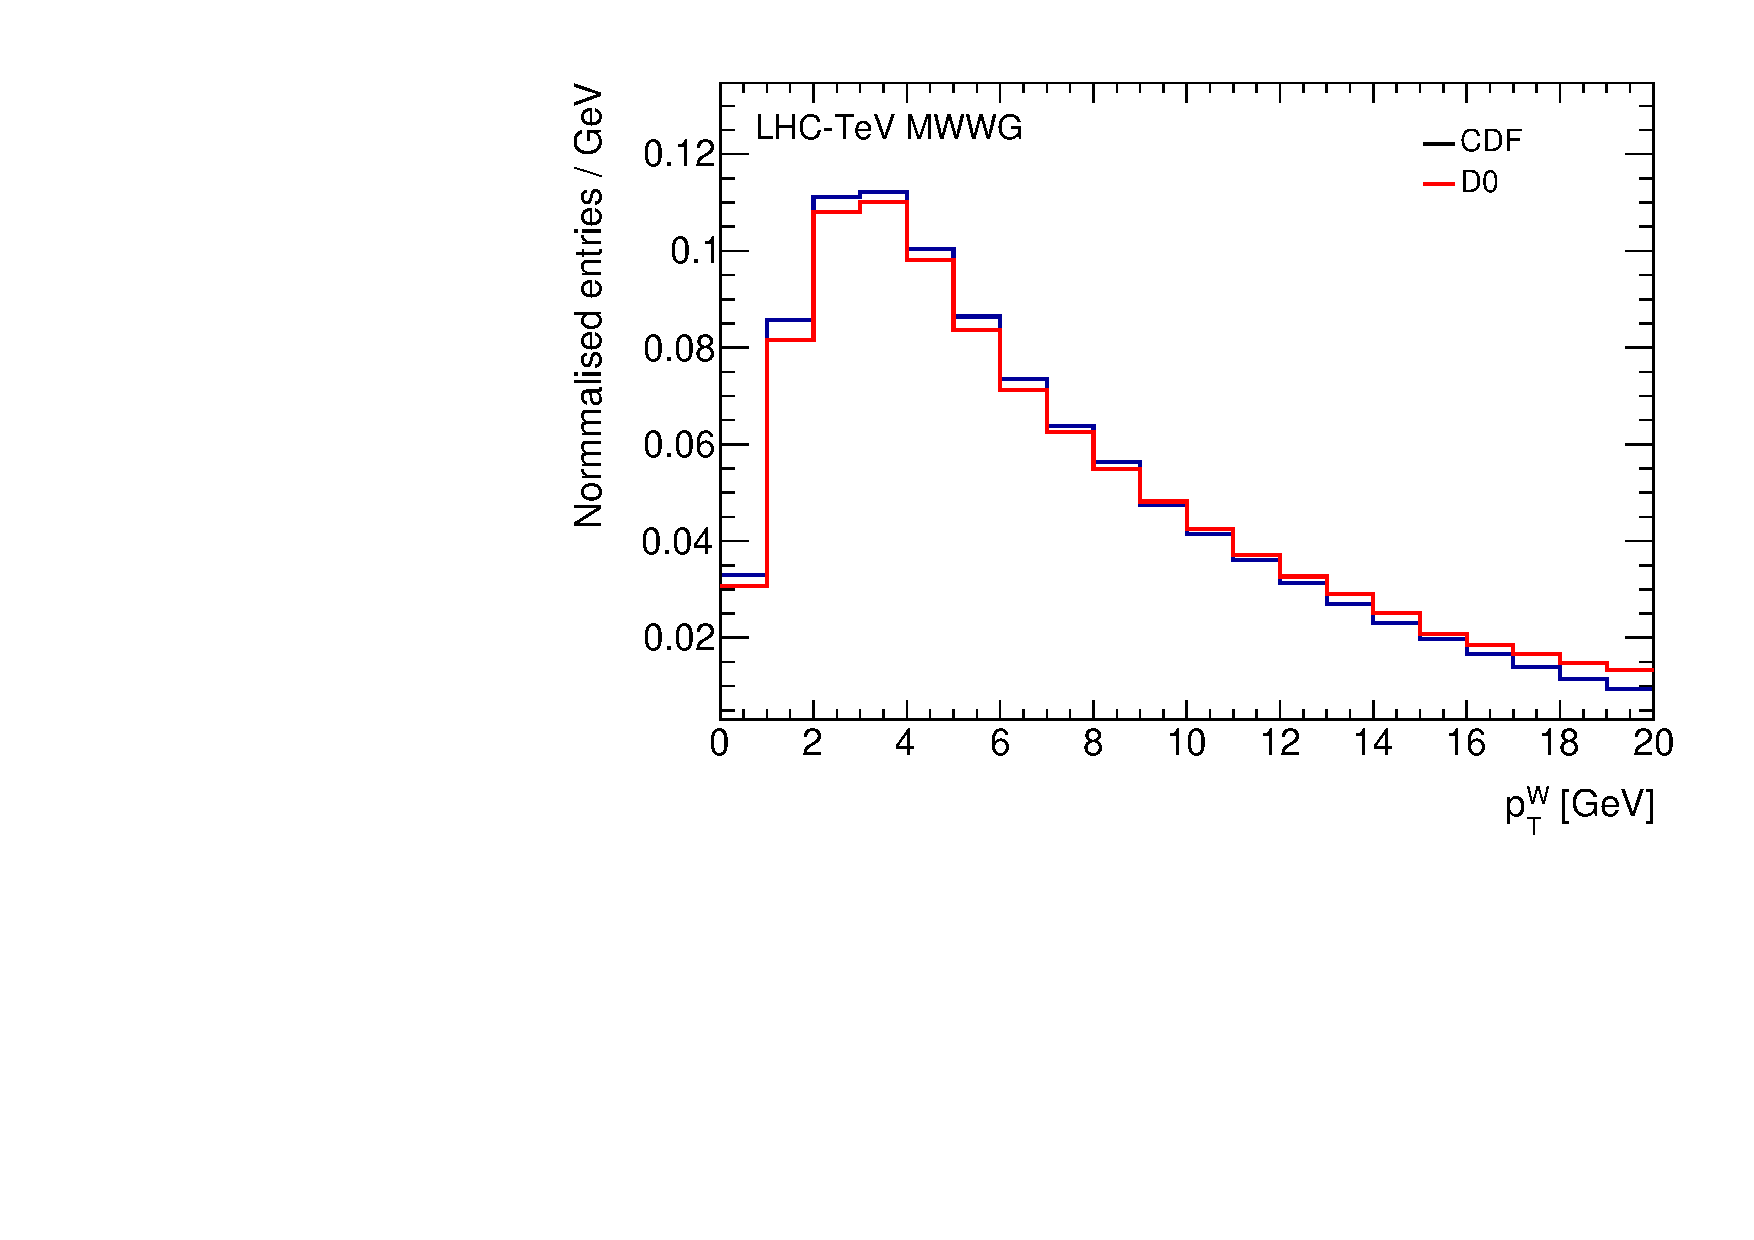
\includegraphics[width=0.9\columnwidth]{pTref_TeV.pdf}
  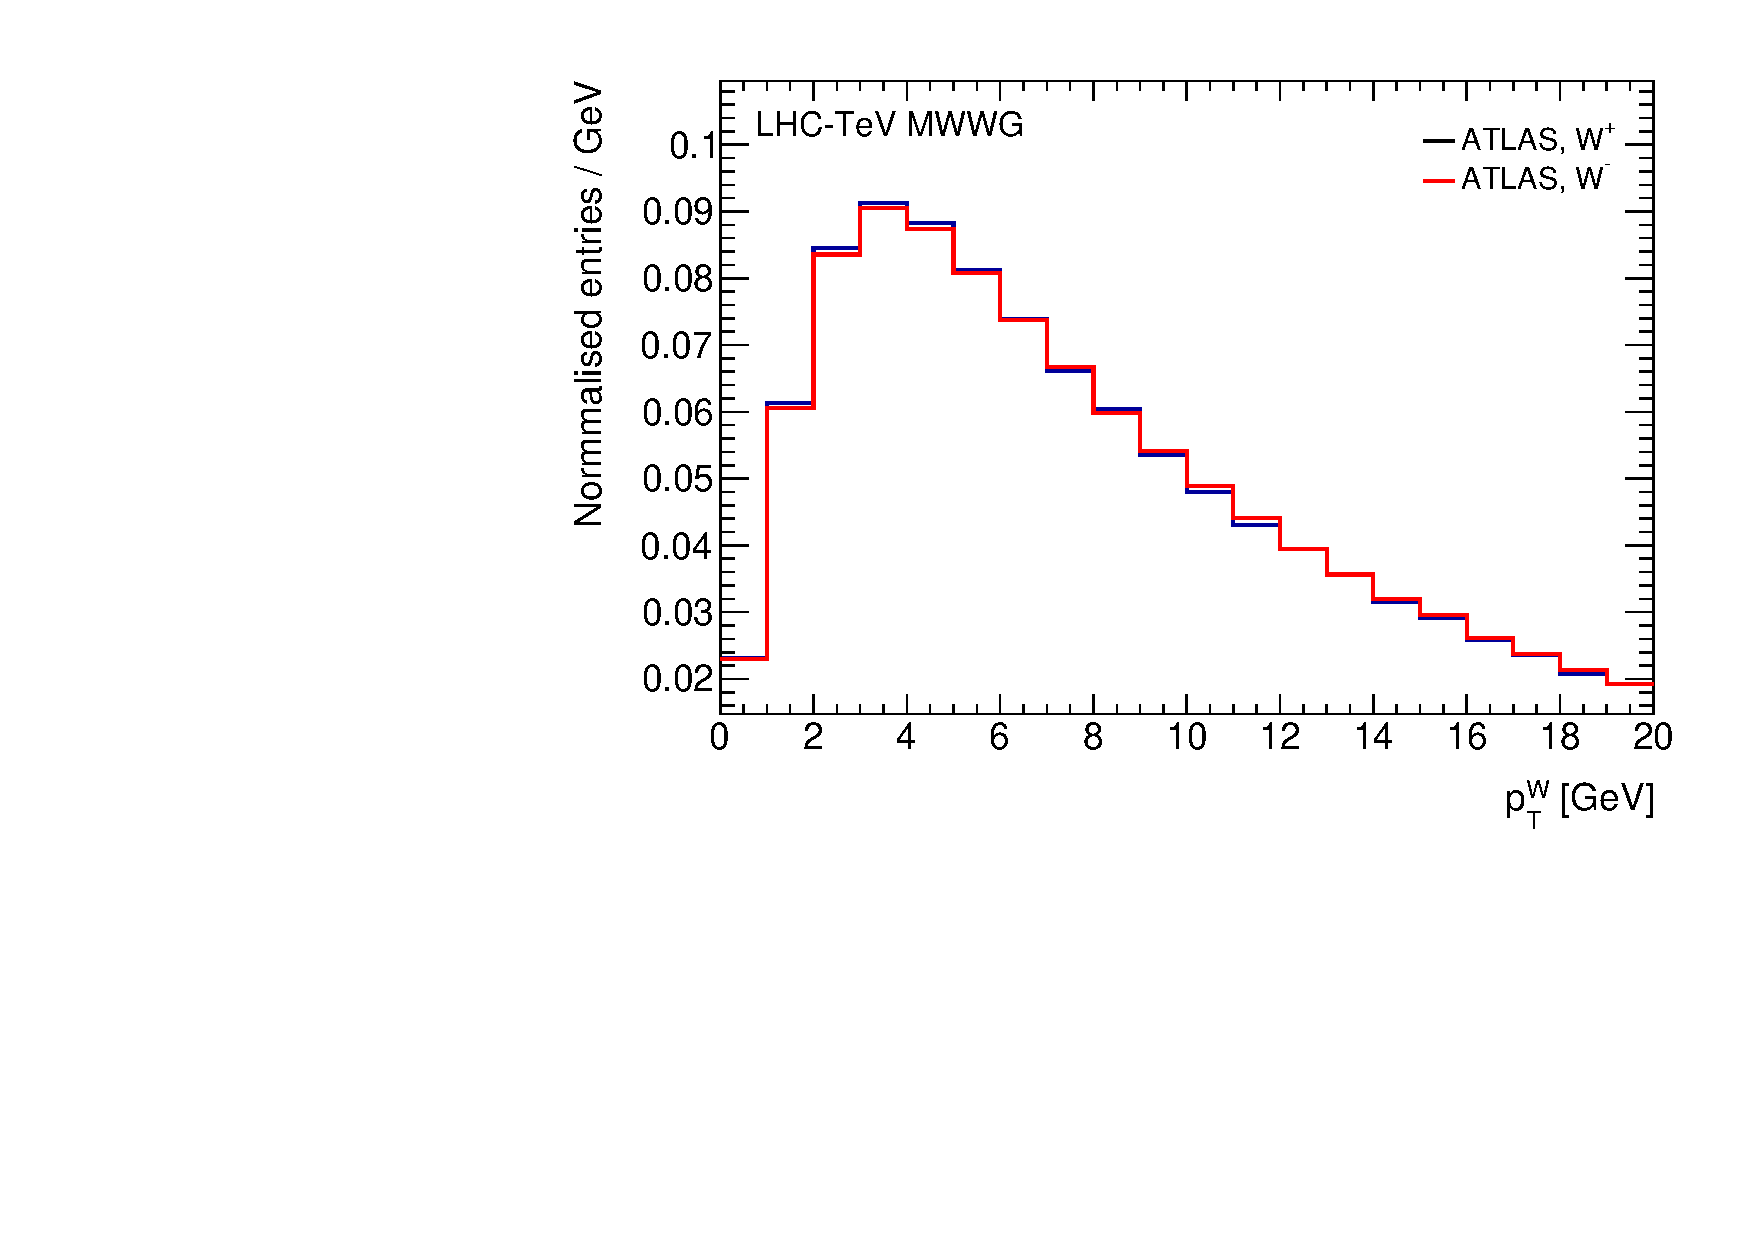
\includegraphics[width=0.9\columnwidth]{refPt_LHC.pdf}
  \caption{Distributions of generated \pTW for $W^\pm$ candidate events in $p\bar{p}$ collisions at CDF and D0 (top), 
and for $W^+$ and $W^-$ events at ATLAS (bottom).  The distributions represent the best-fit model resulting from the 
analysis of $W$- and $Z$-boson data in the respective experiments, and are shown after all event selection requirements. 
\label{fig:ptwmodels}}
\end{figure}

